\section{Numerical Results}
\label{sec:numerical}

In this section, we demonstrate the analytical
claims above with numerical examples and
highlight the performance of the BIE approach
to Stokes eigenvalues.

\subsection{Numerical methods}

First, we describe the numerical tools needed
to compute Stokes eigenvalues in a BIE
framework.

\subsubsection{Discretizing the BIE}

In order to turn the BIEs analyzed
above into discrete linear systems,
we require some standard techniques
from the BIE literature.

Let the boundary be divided into $N_p$
panels.
%
We parameterize panel $j$ as
$\bx_j(t)$, with $t$ ranging over the
interval $[-1,1]$.
%
Each component of $\bx_j$ is taken to be
a polynomial interpolant over the
standard 16th-order Legendre nodes on
$[-1,1]$, denoted by $t_n$, so that
the total number of discretization
points is $N=16N_p$.
%
See \cref{fig:panels} for an example
discretization.
%
Another important quantity below is the
arc-length density of a panel, which
we denote by $s_j(t) := |\bx'_j(t)|$.
%
Finally, we denote the set of panels
which are adjacent to panel $j$
by $A(j)$. On a closed curve,
$A(j)$ contains two integers.

The integral kernels of the single and
double layer potentials have weak
singularities of the form $r^p\log r$
which require special quadrature rules to
achieve high-order accuracy.
%
In the examples below, we use generalized
Gaussian quadrature (GGQ)~\cite{bremer2010}.
%
To demonstrate the idea, we consider
evaluating the convolution of a kernel
$K$ with a density $\sigma$
at the boundary node $\xx_j(t_l)$.
%
GGQ is a Nystr\"{o}m-type discretization ---
the density is approximated 
by its values at the discretization nodes,
which we denote by
$\sigma_{qp} := \sigma(\xx_q(t_p))$.
%
The basis of a GGQ rule is a set of 
support nodes and weights for the
contribution to the integral from the
``self'' panel (panel $j$) and the adjacent
panels (with index in $A(j)$).
%

For the self panel, there is a special set
of nodes and weights for each interpolation
point. Denote the nodes and weights
for interpolation point $l$ by $t^{(l)}_{n}$
and $w^{(l)}_{n}$, respectively, with
$1\leq l \leq 16$ and $1\leq n \leq N_s$.
%
The adjacent panels are handled by a single
set of over-sampled support nodes and weights.
We denote these nodes and weights
by $\tilde{t}_n$ and $\tilde{w}_n$, respectively,
for $1 \leq n \leq N_a$.
%
For the rules we used, $N_s = 16$ and
$N_a = 48$.
%
The contribution of other panels is assumed
to be given to high accuracy by the standard
Gauss-Legendre weights, which we denote
by $w_n$.
%
Adding these contributions together, we obtain the
quadrature

\begin{multline}
  \int_\Gamma K(\xx_i(t_l),\yy) \, \sigma(\yy)
  \, dS(\yy) \approx \\
  \sum_{p=1}^{16} \sum_{n=1}^{N_s}
  w^{(l)}_{n} K(\xx_i(t_l),\xx_i({t}^{(l)}_{n}))
  s_i({t}^{(l)}_{n}) B^{(l)}_{np} \sigma_{ip} \quad \textrm{(self)}
  \\
  + \sum_{q\in A(i)} \sum_{p=1}^{16} \sum_{n=1}^{N_a}
  \tilde{w}_jK(\xx_i(t_l),\xx_q(\tilde{t}_n)) s_q(\tilde{t}_n)
  C_{np} \sigma_{qp}
  \quad \textrm{(adjacent)} \\
  + \sum_{q\neq i, q\not\in A(i)} \sum_{p=1}^{16}
  w_p K(\xx_i(t_l),\xx_q(t_p)) s_q(t_p)
  \sigma_{qp} \quad \textrm{(far)} \nonumber \; ,
\end{multline}
where $\bB^{(l)}$ and $\bC$ are interpolation
matrices from the standard Legendre nodes
to the self and adjacent panel support nodes,
respectively. Observe that the quadrature is
linear in $\sigma_{qp}$. In practice, we pre-compute
and store the self and adjacent matrix entries for each
interpolation point, which is a parallelizable
$O(N)$ calculation. The ``far'' interactions
are computed on-the-fly.

\begin{remark}
  \label{rmk:levelrestrict}
  We ensure that ``far'' interactions
  are handled to high precision by requiring that
  no two adjacent panels differ in length
  by more than a factor of 2. On a domain which does
  not nearly self-intersect this
  guarantees that no ``far'' interactions occur
  which are much closer than 1/2 of a panel away
  (assuming panels are relatively flat).
  Because the location of the singularity is
  bounded away from the panel and the smooth
  rule is of high order, we obtain a quadrature
  rule with sufficient precision.
\end{remark}

\subsubsection{Fast determinant method}

Once the discretization is set, we can form
a compressed representation of the system matrix
using recursive skeletonization~\cite{ho2012fast}.
%
We use the implementation of this procedure
included in the fast linear algebra in
MATLAB (\texttt{FLAM}) package
\cite{hoFLAM_1253582}.
%
At low-to-medium frequencies, the scaling
of the recursive skeletonization algorithm
is $O(N\log N)$ in operation count and
storage and, by using a generalization
of the Sylvester determinant formula,
allows for a fast determinant
calculation in $O(N\log N)$ time as a
follow-up step.
%
At higher-frequencies,
the recursive skeletonization procedure,
which is based on the assumption that off-diagonal
blocks of the matrix are of low rank,
breaks down and does not offer a speed advantage.
%
These algorithms take a precision parameter
$\epsflam$ which determines the
accuracy to which any sub-blocks of the matrix
should be compressed. In all experiments,
we set $\epsflam = 10^{-14}$.

The compressed representation also allows
for fast applications of the system matrix,
its transpose, the inverse of the system
matrix, and the inverse transpose to
vectors.
%
In particular, this allows us to estimate the
smallest singular values by performing
randomized subspace iteration, see
\cite[Algorithm 4.4]{halko2011finding},
on the inverse operator.
%
Below, we use the smallest singular value
as a measure of the quality of the
eigenvalues found by approximating the
roots of the determinant.
%
We also evaluate the second smallest singular
value if the root finding precedure suggests a
possible double root. 

\subsubsection{Interpolation and root-finding}

To estimate the eigenvalues, we fit a Chebyshev
interpolant to the discretized determinant as a
function of $k$ on intervals.
%
This is done adaptively so that the Chebyshev
coefficients of the determinant have decayed
to the point that the ratio of the last
coefficient to the largest coefficient is below
some threshold.
%
In all experiments, we set this threshold
as $\epscheb = 10^{-13}$.
%
We perform this fit using the \texttt{chebfun}
utility in the package of the same name
\cite{driscoll2014chebfun}
so that we can make use
of the \texttt{roots} utility to approximate
the roots of the determinant.

The \texttt{roots} utility returns the roots
of the polynomial in the complex plane, with
some minimal internal processing to remove
spurious roots.
%
Because our numerical determinant evaluation
is somewhat noisy and we fit the function up to
precision $\epscheb$, we perform some
further post-processing to eliminate remaining
spurious roots.
%
Let $k^{(l)}_\cheb$ denote the roots of the interpolants.
%
We ignore any of the returned roots with $|\imag(k^{(l)}_\cheb)|
> \sqrt{\epscheb}$, as these are too far from real-valued
to be non-spurious.
%
For the remaining roots, we consider the
properties of $\real(k^{(l)}_\cheb)$.
%
We inspect any pairs of roots $(k^{(p)}_\cheb,k^{(q)}_\cheb)$
for which $|\real(k^{(p)}_\cheb-k^{(q)}_\cheb)| < \sqrt{\epscheb}$,
as these are possibly spurious double roots.
%
For these pairs, we compare the right singular
vector of the appropriate BIE operator corresponding
to the smallest singular value for each of $\real(k^{(p)}_\cheb)$
and $\real(k^{(q)}_\cheb)$, which we denote by
$\bv_p$ and $\bv_q$.
%
If $\|\bv_p - \bv_q \bv_q^* \bv_p \| < 10^{-5}$, then
we consider the pair to be spurious.
%
For these near double roots, we also check
that there is no two dimensional null-space
corresponding to the root by estimating the
second smallest singular value of the BIE operator.
%
If this is larger than $10^{-5}$, then we declare
it to be a simple root.

We can obtain an a posteriori estimate of the
error in a computed root as follows.
%
Let $f$ denote an analytic function,
$P$ be the polynomial interpolant
of that function over some interval,
$\delta f = f-P$ be the difference,
and $k_\cheb$ denote a computed root
of $P$.
%
The algorithm used by \texttt{chebfun}
to approximate the roots of $P$ is
backward stable~\cite{noferini2017chebyshev}.
Therefore the error in the roots will be
small relative to the error of the fit and
we set $P(k_\cheb) = 0$ below.
%
Suppose that
$f(k_\cheb + \delta k) = 0$ for some
small $\delta k$. Then

\begin{align*}
  0 &= f(k_\cheb + \delta k) \\
  0 &= P(k_\cheb + \delta k) + \delta f(k_\cheb + \delta k) \\
  \delta k &= -\frac{\delta f(k_\cheb + \delta k)}{P'(k_\cheb)} + O(\delta k^2) .
\end{align*}
In practice, we can obtain an approximate upper
bound for $|\delta f(k_\cheb+\delta k)|$
as $\epscheb \|P\|_\infty$ so that $\epscheb \|P\|_\infty/
|P'(k_\cheb)|$ provides an approximate upper bound
for the error in the root.

\subsection{Eigenvalues of an annulus}

\subsubsection{Spurious eigenvalues}
\label{subsec:spurannulus}



\subsubsection{Convergence study}
\label{subsec:convannulus}

\subsection{Eigenvalues of a barbell-shaped domain}
\label{subsec:barbell}

\begin{figure}
  \centering
  \begin{subfigure}[t]{0.4\textwidth}
    \centering
    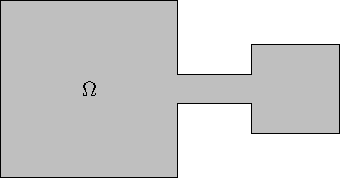
\includegraphics[width=\textwidth]{fig/ex_barbell_001_bdry}
    \caption{A barbell-shaped domain.}
    \label{subfig:barbell_bdry}
  \end{subfigure}
  ~
  \begin{subfigure}[t]{0.4\textwidth}
    \centering
    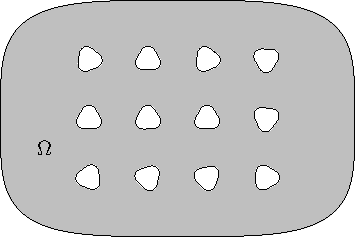
\includegraphics[width=\textwidth]{fig/ex_many_holes_004_bdry}
    \caption{A domain with several inclusions.}
    \label{subfig:many_inclusions_bdry}
  \end{subfigure}
\end{figure}

\begin{figure}
  \centering
  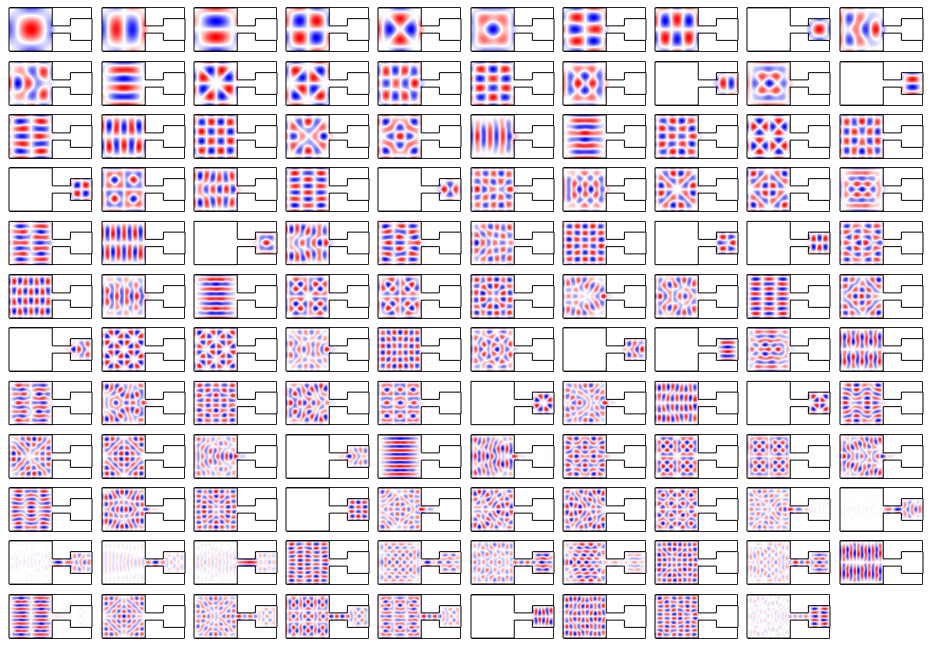
\includegraphics[width=\textwidth]{fig/barbell_gallery}
  \caption{Vorticity plots of the first 119 eigenfunctions
    of the barbell-shaped domain.}
  \label{fig:barbell_gallery}
\end{figure}

\begin{figure}
  \centering
  \begin{subfigure}[t]{0.4\textwidth}
    \centering
    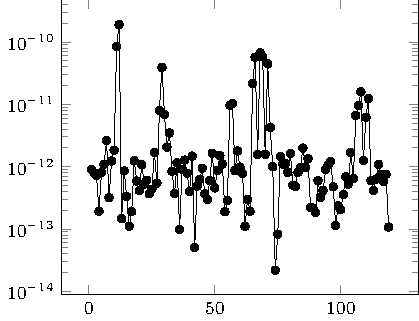
\includegraphics[width=\textwidth]{fig/ex_barbell_001_sings_plot}
    \caption{Smallest singular value of the BIE operator.}
    \label{subfig:barbell_sings}
  \end{subfigure}
  ~
  \begin{subfigure}[t]{0.4\textwidth}
    \centering
    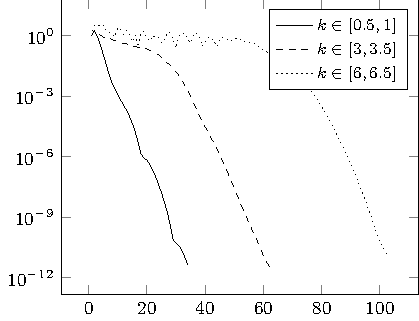
\includegraphics[width=\textwidth]{fig/ex_barbell_001_coeffs_plot}
    \caption{Normalized Chebyshev coefficients of the
      determinant on 3 intervals in $k$.}
    \label{subfig:barbell_coeffs}
  \end{subfigure}
  \caption{Diagnostics for the first 119 barbell eigenvalues.}
  \label{fig:barbell_diagnostics}
\end{figure}

We consider the barbell-shaped domain in \cref{subfig:barbell_bdry}.
This domain is the union of a square of side-length 6,
a square of side-length 3, and a ``bridge'' connecting
them of height 1 and width 5/2.
%
For the sake of simplicity, we round the corners of the domain
to obtain a smooth object.
%
Applying the approach described in~\cite{epstein2016smoothed},
the corners of the domain are rounded by convolving with
the Gaussian kernel
\begin{equation}
  \nonumber
\phi(x) = \frac{1}{\sqrt{2\pi h}} e^{-x^2/(2 h^2)} \, ,
\end{equation}
with $h\approx 0.06$. This leaves the domain unperturbed
to high precision outside of a radius of $0.1$ around
each corner.
%
The eigenfunctions of such a domain display the well-known
localization property~\cite{trefethen2006computed}:
many of the eigenfunctions are approximately supported
within one of the squares.
%
We compute these eigenfunctions corresponding to
eigenvalues $k^2$ with $k$ in the range
$0.5 \leq k \leq 6.5$.

%
The panels are divided adaptively so that the smallest
panels in the rounded corners are smaller than $10^{-2}$,
which keeps the panels relatively flat.
%
This results in $N_p = 412$ after enforcing the
level-restriction property described in
\cref{rmk:levelrestrict}
and enforcing that no panel is larger than
one wavelength for the largest $k$
(here $\lambda=2\pi/6.5$).

As this is a simply-connected domain,
the eigenvalues are estimated by finding the values
$k$ for which $\cI-2\cDk-2\cW$ is non-invertible.
%
Let $f^N(k) = \det (\cI^N-2\cDk^N-2\cW^N)$.
To find the roots of $f^N(k)$, we fit a \texttt{chebfun}
representation of $f^N(k)$ on each of the intervals
$[j/2,(j+1)/2]$ for $j = 1,\ldots,12$.
%
We plot the absolute value of the Chebyshev coefficients
(normalized by the absolute value of the first coefficient)
of $f^N(k)$ on the intervals $[0.5,1.0]$, $[3.0,3.5]$,
and $[6.0,6.5]$ in \cref{subfig:barbell_coeffs}.
%
As expected, the coefficients decay exponentially
to zero, with more terms required at higher
frequencies.
%

We compute the roots of these Chebyshev interpolants
and apply the post-processing described above.
%
There were 135 total roots: 3 were removed because
the imaginary part was too large and 13 pairs were found
with values within $\sqrt{\epscheb}$ of each other.
%
For these 13 pairs, none represented two distinct
eigenvalues or a double root.
%
This leaves 119 roots in the range $0\leq k \leq 6.5$.
%
We plot the smallest singular value of
$\cI^N-\cDk^N-2\cW^N$ for each of these roots in
\cref{subfig:barbell_sings}
and plot the vorticity of the eigenfunctions
in \cref{fig:barbell_gallery}.
%
The singular values suggest that the quality of the
eigenvalues is good.
From the plots, we see that localization occurs
until about the 100th eigenvalue.

%

%\subsection{Robustness on a nearly multiply connected domain}
%\label{subsec:crescent}

\subsection{Eigenvalues of a domain with several inclusions}

\begin{figure}
  \centering
  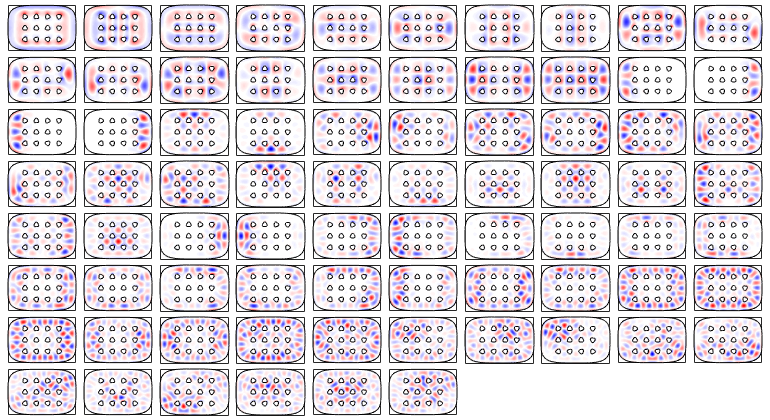
\includegraphics[width=\textwidth]{fig/many_inclusions_gallery}
  \caption{Vorticity plots of the eigenfunctions corresponding
  to the first 76 eigenvalues of a domain with several inclusions.}
  \label{fig:many_inclusions_gallery}
\end{figure}

\begin{figure}
  \centering
  \begin{subfigure}[t]{0.4\textwidth}
    \centering
    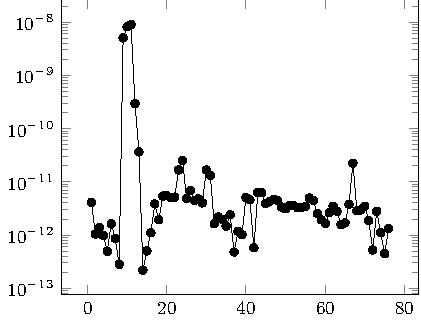
\includegraphics[width=\textwidth]{fig/ex_many_holes_004_sings_plot}
    \caption{Smallest singular value of the BIE operator
      corresponding to the first 76 eigenvalues of a
      domain with several inclusions.}
    \label{subfig:many_inclusions_sings}
  \end{subfigure}
  ~
  \begin{subfigure}[t]{0.4\textwidth}
    \centering
    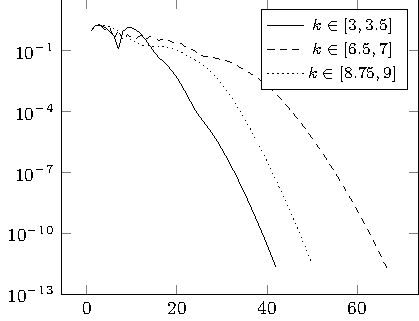
\includegraphics[width=\textwidth]{fig/ex_many_holes_004_coeffs_plot}
    \caption{Normalized Chebyshev coefficients of $f^N(k)$ on
      3 different intervals in $k$.}
    \label{subfig:many_inclusions_coeffs}
  \end{subfigure}
  \caption{Diagnostics for the eigenvalues of a domain
    with several inclusions.}
  \label{fig:many_inclusions_diagnostics}
\end{figure}

We now consider the multiply-connected domain in
\cref{subfig:many_inclusions_bdry}.
% 
The domain is defined by a smooth rectangular region
of width 3 and height 2,
with an array of randomly rotated ``starfish'' shapes
removed. 
%
Such shapes are of interest in
materials design and micro-fluidics \note{cite}.
%
We compute the eigenfunctions corresponding to
eigenvalues $k^2$ with $k$ in the range
$3 \leq k \leq 9$ (this range includes the smallest
eigenvalue).

%
For this smooth shape, ensuring that no panel is
larger than one wavelength for the largest $k$
(here $\lambda=2\pi/9$) is sufficient to resolve
the object to high precision.
%
After enforcing the
level-restriction property described in
\cref{rmk:levelrestrict}, we end up with
$N_p = 224$.

As this is a multiply-connected domain,
the eigenvalues are estimated by finding the values
$k$ for which $\cI-2\cDk-2i\cSk-2\cW$ is non-invertible.
%
Let $f^N(k) = \det (\cI^N-2\cDk^N-2i\cSk^N-2\cW^N)$.
To find the roots of $f^N(k)$, we fit a \texttt{chebfun}
representation of $f^N(k)$ on each of the intervals
$[j/2,(j+1)/2]$ for $j = 6,\ldots,13$ and the intervals
$[j/4,(j+1)/4]$ for $j = 28,\ldots,35$.
%
It should be noted that, due to the relative sizes
of the domains,
this represents a lower frequency problem than
that for the barbell when measured in the number
of wavelengths across the object.
%
Thus, the use of a finer grid in frequency results from
the difficulty in resolving the Fredholm determinant
for this problem, which has a larger dynamical range
than that for the barbell.
%
We plot the absolute value of the Chebyshev coefficients
of $f^N(k)$ on the intervals $[3,3.5]$, $[6.5,7]$,
and $[8.75,9]$ in \cref{subfig:barbell_coeffs}.
%
As expected, the coefficients decay exponentially
to zero, with more terms required at higher
frequencies (note that the interval $[8.75,9]$ is
smaller than the others).
%

We compute the roots of these Chebyshev interpolants
and apply the post-processing described above.
%
There were 103 total roots: 21 were removed because
the imaginary part was too large and 6 pairs were found
with values within $\sqrt{\epscheb}$ of each other.
%
For these 6 pairs, none represented two distinct
eigenvalues or a double root.
%
This leaves 76 roots in the range $0\leq k \leq 9$.
%
We plot the smallest singular value of
$\cI^N-\cDk^N-2i\cSk^N-2\cW^N$ for each of these roots in
\cref{subfig:many_inclusions_sings}
and plot the vorticity of the eigenfunctions
in \cref{fig:many_inclusions_gallery}.
%
In the vorticity plots, we observe a different type of
localization property than that seen in the barbell,
with many of the eigenfunctions
approximately supported in a small, connected subset
of the domain. This is consistent with other studies
\note{cite}

%

\begin{figure}
  \centering
  \begin{subfigure}[t]{0.4\textwidth}
    \centering
    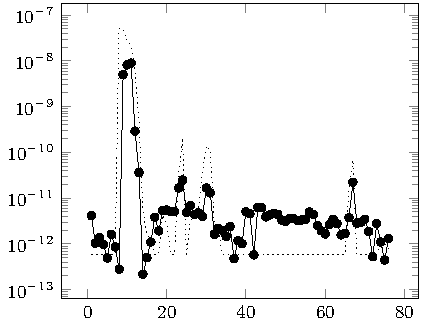
\includegraphics[width=\textwidth]{fig/ex_many_holes_004_sings_plot_west}
    \caption{Smallest singular value of the BIE operator
      for the computed roots (original intervals)
      along with an estimate of the error in the root (dotted).}
    \label{subfig:many_inclusions_sings_west}
  \end{subfigure}
  ~
  \begin{subfigure}[t]{0.4\textwidth}
    \centering
    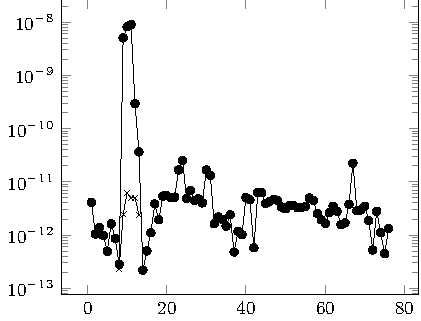
\includegraphics[width=\textwidth]{fig/ex_many_holes_004_sings_plot_ref}
    \caption{Smallest singular value of the BIE operator
      for the computed roots on the original intervals (\textbullet)
      and the values obtained on the refined interval ($\times$).}
    \label{subfig:many_inclusions_sings_ref}
  \end{subfigure}
  \caption{Further diagnostics for the eigenvalues of a domain
    with several inclusions.}
  \label{fig:many_inclusions_diagnostics_2}
\end{figure}

The singular values suggest that the quality of the
eigenvalues is good, with a few outliers.
%
To explain these outliers, we consider two quantities
which affect the singular value at a computed root.
%
As described above, we can approximate the
error in the computed root at $k_\cheb$ by
$\epscheb \|P\|_\infty/|P'(k_\cheb)|$,
where $P$ is the interpolating polynomial.
%
The singular value estimate itself is affected by
the error incurred in applying the inverse of the
compressed BIE matrix, which can be hard to quantify
\cite{ho2012fast}.
%
We approximate this error by $O(\sqrt{N})\epsflam$
and assume this is the order of the error in
the singular value estimate.
We plot the maximum of these two estimates
along with the computed singular values in
\cref{subfig:many_inclusions_sings_west}.
There is a reasonably good correlation between
the maximum of the error estimates and the
observed smallest singular value for the BIE,
especially for larger errors.

The worst outliers are from the left half
of the interval $[4.5,5]$.
%
Because the determinant is much larger on the
right half than the left half of $[4.5,5]$,
we can improve the estimate for the error
in the roots by subdividing the interval. 
We plot the smallest singular value of the
BIE for the roots obtained by fitting a polynomial
on $[4.5,4.75]$ in \cref{subfig:many_inclusions_sings_ref};
the roots on the refined interval
are of significantly higher quality.

\begin{remark}
  The above experience suggests that
  the ratio $\|P\|_\infty/|P'(k_\cheb)|$
  is a useful diagnostic for performing
  automated eigenvalue estimation.
  Note that at a multiple root, this ratio
  will be more difficult to bound.
\end{remark}
%



%
